\documentclass[letter, USenglish, 11pt, subfigure]{article}
\usepackage[margin=1in]{geometry}
\newcommand*{\ATLASLATEXPATH}{./}
\usepackage{\ATLASLATEXPATH atlaspackage}
\usepackage{\ATLASLATEXPATH atlasbiblatex}
\usepackage{\ATLASLATEXPATH atlasphysics}
\usepackage{\ATLASLATEXPATH ANA-SUSY-2018-12-PAPER-defs}
\usepackage{enumerate}
\usepackage{caption, float, threeparttable}
\newcommand{\tth}{\ensuremath{\ttbar H}}
\newcommand{\ttH}{\ensuremath{\ttbar H}}
\newcommand{\tthyy}{\ensuremath{\ttbar H(\to\gamma\gamma)}}
\newcommand{\myy}{\ensuremath{m_{\gamma\gamma)}}}
\newcommand{\hyy}{\ensuremath{H(\to\gamma\gamma)}}

\usepackage{lineno}

\linenumbers
\usepackage{wrapfig}
\usepackage{placeins}
\usepackage{pdfpages}
\usepackage[none]{hyphenat}

\usepackage{xifthen}
\usepackage{multirow,bigdelim,makecell}
\usepackage{cellspace}
\usepackage{selectp}
\usepackage{color, colortbl}

% \outputonly{1}
\usepackage[nottoc,numbib]{tocbibind}

\addbibresource{proposal_WHopkins.bib}
\addbibresource{ATLAS-SUSY.bib}
\addbibresource{ATLAS.bib}
\addbibresource{ANA-HDBS-2021-10-PAPER.bib}
\addbibresource{CMS.bib}

\pagestyle{headings}

\title{Early Career Research Proposal: \\Enabling Calibrations of Machine Learning Approaches (ECMLA)}
\author{Applicant/Institution: Walter Hopkins, Argonne National Laboratory\\ Postal Address: \\Argonne National Laboratory, 9700 S. Cass Avenue, Building 360, Lemont, IL 60439
  \\PI name: Walter Hopkins\\Position title for PI: Physicist\\PI telephone number, email: (630) 252 7551, whopkins@anl.gov\\Administrative Point of Contact name, telephone number, email:\\Diane Hart, (630) 252 7677, dhart@anl.gov\\FOA Number: DE-FOA-0003176\\DOE/SC Program Office: HEP\\ Topic Area: Experimental Research at the \\Energy Frontier in High Energy Physics\\DOE/SC Program Office Technical Contact: Abid Patwa\\Year Doctorate Awarded: 2013\\Number of Times Previously Applied: 2\\Eligibility Extension Requested: No
}
\date{}

\begin{document}
\pagenumbering{gobble}
% \includepdf{cover_page_signed.pdf}

% \maketitle
\clearpage
\tableofcontents
\thispagestyle{empty}

\clearpage
\pagenumbering{arabic} 

% eBUD proposal ID: 39999.1

\section{Introduction}

% chatGPT rewrite (which is a little too dreamy):
% Machine Learning (ML) has swiftly risen to prominence within the realm of High-Energy Physics (HEP), marking a transformative era in the field's methodological arsenal. Its application spans an impressive spectrum of tasks, from simulating calorimeter showers to the nuanced identification of particles such as photons and electrons, and the critical differentiation between signal and background processes. This technological evolution enables physicists to extract and leverage complex correlations across an extensive array of observables, including but not limited to particle four-vectors and energy depositions in calorimeters. These advancements underscore the potential of ML to significantly enhance analytical precision and efficiency in HEP research.

% Nonetheless, the integration of ML within HEP is not without its challenges. A notable concern arises from the input variables to ML algorithms, where discrepancies in distributions between Monte Carlo (MC) simulations and actual experimental data can lead to mismodelling by the ML models themselves. Such discrepancies, even when marginal, can amplify uncertainties in the outcomes of these algorithms, thereby impacting the reliability and robustness of the research findings. Moreover, ML models possess the capacity to inadvertently introduce correlations between the predicted targets—be it estimated energy levels or particle type classifications—and variables integral to calibration processes or background estimations. This phenomenon could potentially skew the interpretative accuracy of the results and necessitate sophisticated approaches to mitigate its effects.

% The dialogue between ML advancements and HEP research thus unfolds as a narrative of progress shadowed by the imperative for meticulous validation and calibration. It underscores the need for ongoing innovation in algorithmic design and training methodologies that are attuned to the intricacies of HEP data, ensuring that ML models not only enhance the analytical capabilities of physicists but also uphold the stringent standards of precision and accuracy foundational to the field.


% Slightly toned down version
% Machine learning (ML) has increasingly become a critical tool in High-Energy Physics (HEP), offering significant advancements in various tasks such as simulating calorimeter showers, identifying particles like photons and electrons, and distinguishing between signal and background processes. These ML techniques allow physicists to delve into complex correlations among a wide range of observables, from the trajectories and energies of particles to their interactions within detectors. This integration of ML into HEP has not only streamlined data analysis processes but also opened up new avenues for discovery by exploiting the full potential of available data.

% However, the application of ML in HEP is accompanied by certain challenges that need careful consideration. One such challenge is the alignment of input variable distributions between Monte Carlo (MC) simulations and real experimental data. Discrepancies in these distributions can lead to misinterpretations by the ML models, reflecting the same biases or errors present in the simulations. Even minor differences between the MC simulations and actual data can introduce additional uncertainties into ML predictions, affecting the overall accuracy and reliability of the results.

% Furthermore, ML models can sometimes create unintended correlations between their outputs (such as estimated energy or particle classifications) and other variables critical for calibrations or background estimations. This can complicate the interpretation of results and potentially introduce biases into subsequent analyses.

% Addressing these challenges requires a nuanced approach to ML model development and validation in HEP. It underscores the importance of rigorous testing and calibration of ML algorithms against a backdrop of real-world data, ensuring that these powerful tools contribute positively to the field without compromising the integrity and accuracy of research outcomes.



Machine learning (ML) has become ubiquitous within High-Energy Physics (HEP) and has been used for a range of tasks, including the generation of calorimeter showers, the identification (ID) of particles (i.e., photons and electrons), and the commonplace classification between signal and background processes. These techniques have allowed physicists to take advantage of nuanced correlations from a sometimes large array of observables (e.g., four vectors of particles, energy deposits in calorimeters, etc). However, some input variables, which may result in significant improvements to the performance of an ML algorithm, can have differing distributions when comparing Monte Carlo (MC) simulations and recorded data, which in turn causes the ML model to display the same mismodelling. Even when these data-MC differences are small, they can result in increased uncertainties for the final algorithm. Additionally, ML models could introduce undesirable correlations between the target (e.g., an estimated energy, a classification into different particle types) and variables that are needed for calibrations or background estimations.

Recently proposed adversarial~\cite{louppe2017learning} and distance correlation (DisCo)~\cite{PhysRevLett.125.122001} techniques have shown promise in various applications such as reducing uncertainties in a long-lived particle search~\cite{calRatio}  and decorrelating substructure variables from a jet mass~\cite{ATL-PHYS-PUB-2018-014}. These approaches have the potential to be more broadly applied when developing ML models to estimate physics object properties (e.g., photon energy, jet transerve momentum, etc) or to identify physics objects (e.g., photons, jets containing $b$-hadrons, etc), and to reduce the sensitivity to MC mismodelling for these algorithms, thus reducing the total uncertainties associated with the models. 

This proposal presents {\bf the development of a framework to decorrelate, using multiple approaches such DisCo and adversarial, machine-learning-based physics object identification and property estimation to ensure that ML models are independent from specific quantities and insensitive to regions of kinematic space where quantities are mismodelled. This will maximize ID efficiencies and property estimation precision by making use of all available information that would otherwise be left unused due to mismodelling and calibration concerns.} The proposed techniques could also improve object ID and property evaluations (potentially improving both the efficiency and resolution) at the trigger level, especially given the recent work on fast inference on field-programmable gate arrays (FPGAs).

Improving both ID efficiencies (which is equivalent to recording more data with the same efficiency) and reducing systematic uncertainties will be essential to enabling future discoveries in collider physics.  Results from the Large Hadron Collider (LHC) experiments have verified the predictions of the highly successful Standard Model (SM), culminating with the discovery of the Higgs boson~\cite{HIGG-2012-27,CMS-HIG-12-028}. However, the SM  lacks an explanation for several observed phenomena (e.g., dark matter, the matter-antimatter asymmetry, etc) motivating the search for Beyond the Standard Model (BSM) physics. Future LHC upgrades will no longer include substantial increases in energy and move HEP into the precision era, with a doubling (Run~3) and then a tenfold increase (High Luminosity-LHC, HL-LHC) of the Run~2 data set. 

Precision measurements of SM processes, especially interaction involving Higgs bosons, can probe for BSM effects resulting from particles which may have large masses that prevent them from being directly produced at the LHC. An essential aspect to improving the precision of measurements, which will maximize sensitivity to BSM physics, is the calibration of physics object ID and properties. This calibration involves evaluating ID efficiencies and properties in MC simulations and correcting these quantities to the true property before reconstruction or to what is observed in data. 

The Higgs boson self coupling and the coupling to the top quark are especially sensitive to BSM effects~\cite{Agrawal_2020}. The associative production of a top quark pair with a Higgs boson (\tth) is sensitive to both of these couplings~\cite{Maltoni_2017} and thus the \tth\ total and particularly differential cross section measurements, e.g., as function of Higgs \pt, can serve as probes for BSM physics. The latest ATLAS \hyy, which includes \tthyy, differential cross section results~\cite{ATLAS_STXS} remain limited by the statistical uncertainty in each kinematic observable bin. However, the photon ID and energy resolution uncertainties are the dominant detector-based systematic uncertainties and are currently on par with the other dominant source of systematic uncertainty, theory uncertainties. Reducing these detector systematic uncertainties will become significantly more important for all \hyy\ measurements, as ATLAS drastically increases the size of its data set near the end of HL-LHC data taking. Thus, the unprecedented data volume of the HL-LHC offers an opportunity to improve the precision cross section measurements as a function of kinematic variables in channels with high \tth\ purity, i.e., where the Higgs decays to two photons (\tthyy).

The proposed framework and techniques will first be developed and applied to photon ID and energy resolution because these are key ingredients to maximizing the sensitivity of Higgs precision measurements. Studies have been performed within ATLAS that showed a potential $\sim$10-20\% improvement in both ID efficiency and energy resolution when including all available information for ID and energy estimation. However, as soon as the calibration of the ID efficiency and energy resolution was taken into account, the gain in efficiency and enhancement in resolution were lost. For the ID, ML approaches were found to be correlated with quantities that needed to be independent of the ID for the calibration while for the energy resolution it was found that ML methods were sensitive MC mismodelling of shower shapes. Thus, {\bf the proposed decorrelation techniques could improve all ATLAS measurements involving $H\to\gamma\gamma$ which are essential to the HL-LHC BSM search program.}

The PI's experience in ML, e.g., as one of the ATLAS ML Forum conveners, as well as his experience with the LAr calorimeter and calorimeter simulations will aid the success of this proposal. The PI will also draw from his work within the ATLAS SUSY group, as a leader of flagship searches~\cite{stop0L_1,stopRun1,stop0L_2,stop0L_3} involving $\ttbar$ final states. Additionally, the PI will leverage the computing resources and ML expertise at the Argonne Leadership Computing Facility (ALCF).


\subsection{Background and Motivation}

Machine learning has already been used for the identification of various physics objects (i.e., electrons, jets containing b-hadrons, etc) and to calibrate properties of objects (e.g., for pions~\cite{ATL-PHYS-PUB-2020-018}). Many of these ML models, however, use simulations for training and do not automatically take data and MC differences into account during training. Additionally, algorithms may be required to be independent from variables that are either used in part of the calibration procedure, e.g., to determine the rate of fake objects~\cite{atlas_photon_id}, or that might vary during the operations of the collider or detector, e.g., the number of proton-proton interactions per bunch crossing (pileup) which will be particularly challenging environment at the HL-LHC.

Machine-learning-based photon ID techniques have been studied within ATLAS demonstrating a potential gain in signal efficiency of 5-10\% while retaining the same background rejections as the current rectangular-requirement-based ID. Such an increase in efficiency would impact all $H\to\gamma\gamma$ measurements by improving the statistical power of these measurements with the same amount of HL-LHC data. However, the requirement of orthogonality to particular quantities (i.e., isolation) has limited the use of ML for photon ID within ATLAS. Additionally, the Phase II upgrade of the ATLAS Inner Tracker (ITk) will improve the track isolation (a measure of the energy associated with the candidate vs the energy around the candidate), which is used in the calibration of the photon ID efficiency. This improvement yields an opportunity to revisit the ATLAS photon ID and its calibration to maximize performance during the HL-LHC.

The calibration of photon energies was studied using both advanced ML architectures, i.e., convolutional neural networks (CNNs) and graph neural networks (GNNs), and more information than the current boosted-decision-tree (BDT) based algorithm used. The resulting calibration showed a $\sim$20\% improvement in photon energy resolution but was sensitive to data-MC mismodelling in variables that summarized the shape of the energy deposits in the calorimeter. Ensuring that ML models are invariant with respect to these mismodelled quantities could result in significantly improved photon energy resolution which in turn will reduce the systematic uncertainties for analyses that include photons in their final states.

There have been recent advancements in decorreclating ML models from variables (e.g., jet substructure from jet mass) using methods such as adversarial discriminants and DisCo. 
Adversarial approaches have been deployed to generate data, including calorimeter showers~\cite{calogan,fastsim3}, and involve two ML models, one that generates high-dimensional distributions and another model that is trained to discriminate between the ML-generated data and the real data. More recently, adversarial approaches have been used to discriminate between recorded and simulated data from the output of another discriminator. This strategy, i.e., to use a discriminator to penalize an ML model for giving differing results, can be applied to minimize differences between data and MC and to remove correlations to certain variables by including two loss (i.e., cost) functions, one for each ML model. The two opposing optimizations can, however, cause the training to be compute intensive and make it difficult to determine when to stop training. 
Distance correlation summarizes the dependence of sets of variables and is sensitive to non-linear correlations, which are commonly present in HEP datasets, unlike the more frequently used measure of the Pearson correlation coefficient which can only detect linear correlations. The DisCo is zero only and only if there are no correlations between the input variables. This feature allows it to easily be added to typical loss (or cost) functions which are minimized to optimize ML models. Thus, DisCo is simpler to implement than adversarial techniques with less hyperparameter (since only a loss term is added rather than an entire NN) and more stable training characteristics. % make diagrams
These decorrelation methods allow ML techniques to maximize the use of all information while avoiding regions of kinematic phase space that are poorly modelled in simulation and/or ensure an ML model is independent of a quantity, such as pileup or isolation. Finally, these approaches also avoid regions where there are differences between recorded data and simulations within non-linear correlations. Both adversarial and DisCo approaches can be the optimal solution for a particular application and should be studied to maximize the performance of a particular ML model. The rise of AI/ML-focused High-Performance Computers (HPCs), suchs at Aurora at the ALCF, will facilitate the development of these decorrelation techniques. 

% This may need to be removed
Typically, physics object properties are corrected for differences between MC and data in bins of variables affected by changing detector effects (e.g., the pseudorapidity, $\eta$, and transverse momentum, \pt, of an object). The dimensionality of these bins is limited by practical considerations with the bin edges being chosen manually. Another set of ML techniques, known as clustering, not only allows for an automated way to group similar events at higher dimensions, it also enables correlations between these variables to be taken into account. Clustering has already been used to choose groupings in a two dimensional space for an analysis~\cite{ttH_tau_CMS} and the PI has studied these techniques to group theory models with similar final states. These ML approaches can help not only improve the calibration of physics objects but can also improve the speed of the calibration cycle by automating part of the process.

\begin{figure}[!htbp]  
  \centering
  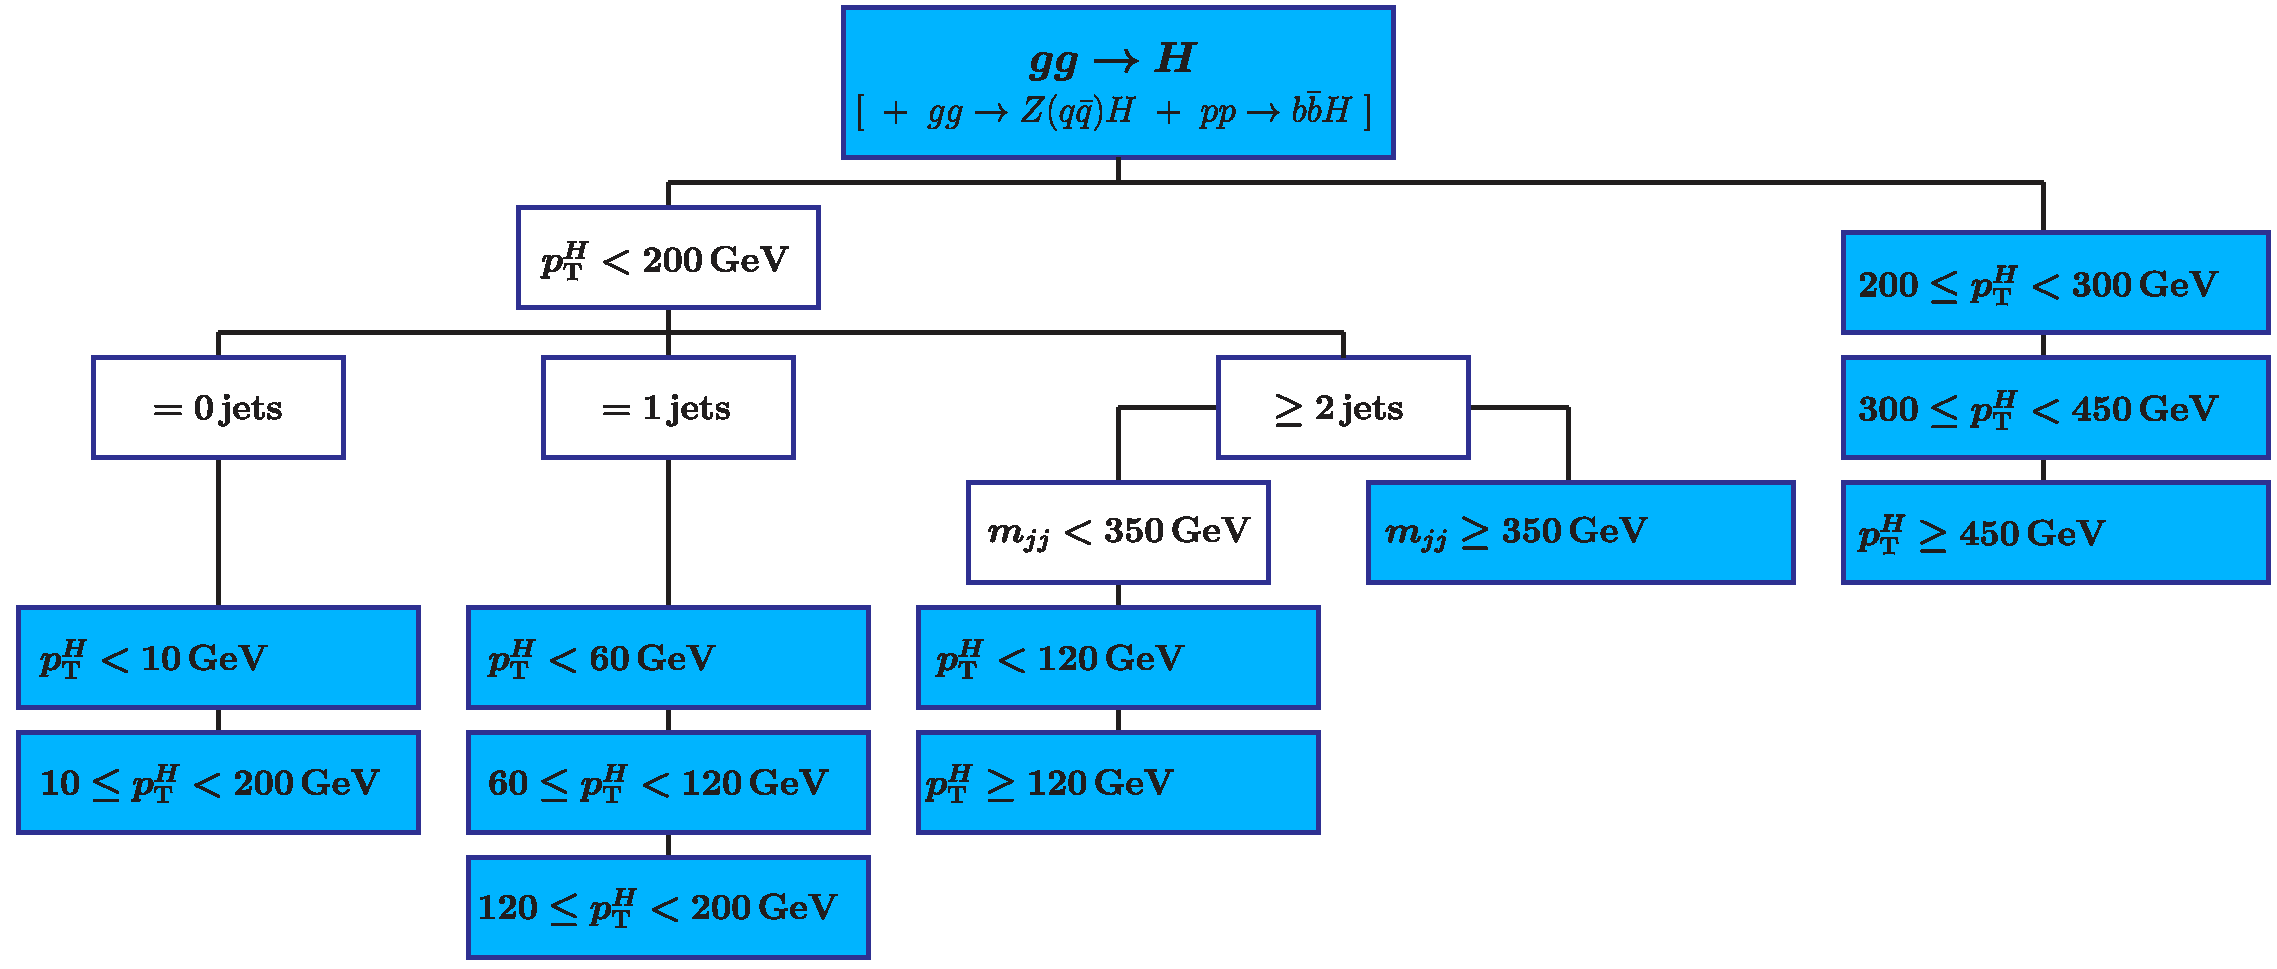
\includegraphics[width=\textwidth]{figures/ggH_STXS.pdf}
  \caption{\label{fig:ggH_STXS} Examples of regions defined by bins in kinematic quantities used to constrain BSM effects in the ATLAS STXS measurement~\cite{ATLAS_STXS} and the gluon-gluon to Higgs channel.}
\end{figure}


The HL-LHC, heralds a new frontier in HEP, characterized by unparalleled precision and voluminous datasets that transition many experiments from being statistically constrained to being dominated by systematic uncertainties. This paradigm shift underscores the pivotal role of systematic uncertainties in shaping the landscape of precision measurements within the HEP domain. 
Measurements, especially those involving the SM Higgs, become increasingly sensitive to high mass BSM contributions as the precision of measurements improves. As the size of the LHC data set grows, differential cross section measurements, which can further expose the effects of BSM physics in high-energy regions (see Figure~\ref{fig:SMEFT_highmass} for an illustration of this effect), become more powerful tools in the search for BSM physics.
\begin{wrapfigure}{l}{0.5\textwidth}
  \centering
  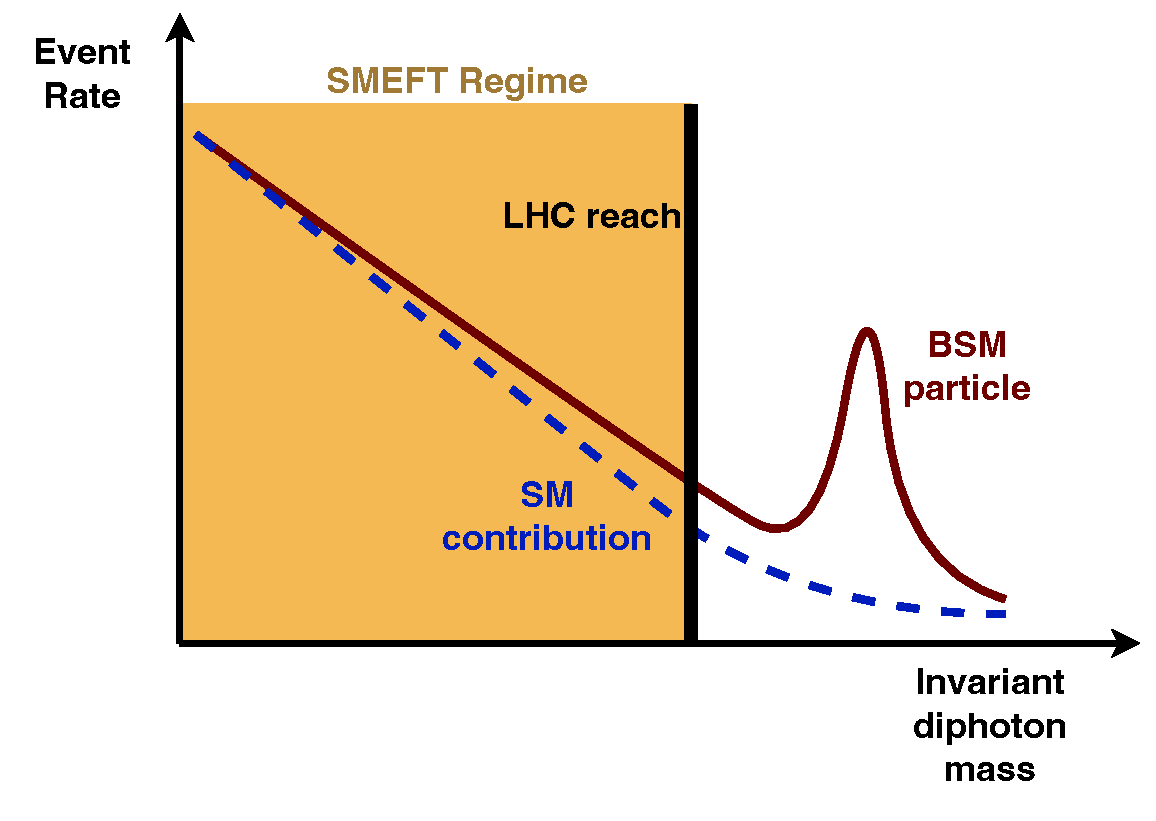
\includegraphics[width=\linewidth]{figures/SMEFT.pdf}
  \caption{\label{fig:SMEFT_highmass} Example of how effects of a heavy BSM particle can leak into high-energy regions of distributions measured at LHC experiments.}
\end{wrapfigure}
The results of differential cross sections measurements can probe BSM effects by being interpreted in the context of the Standard Model Effective Field Theory (SMEFT)~\cite{Buchmuller:1985jz,Grzadkowski:2010es,SMEFTsim3} and in the case of Higgs-related measurements, results can also be interpreted in terms of coupling strengths within the $\kappa$-framework~\cite{deFlorian:2016spz}. An example of a recent differential cross section measurement involving the decay of the SM Higgs to two photons~\cite{ATLAS_STXS} used the simplified cross section template (STXS) method, which performs measurements in bins in several kinematic dimensions (see Figure~\ref{fig:ggH_STXS}) to constrain BSM effects. Current measurements statistically limited but have substantial systematic uncertainties (up to $\sim$40\% in one of the differential cross section bins) which will become crucial in the HL-LHC era. For many of these measurements photon resolution and ID are some of the largest experimental uncertainty (see Figure~\ref{fig:stxs_unc}). 

\begin{figure}[!htbp]  
  \centering
  \subfigure[ggF]{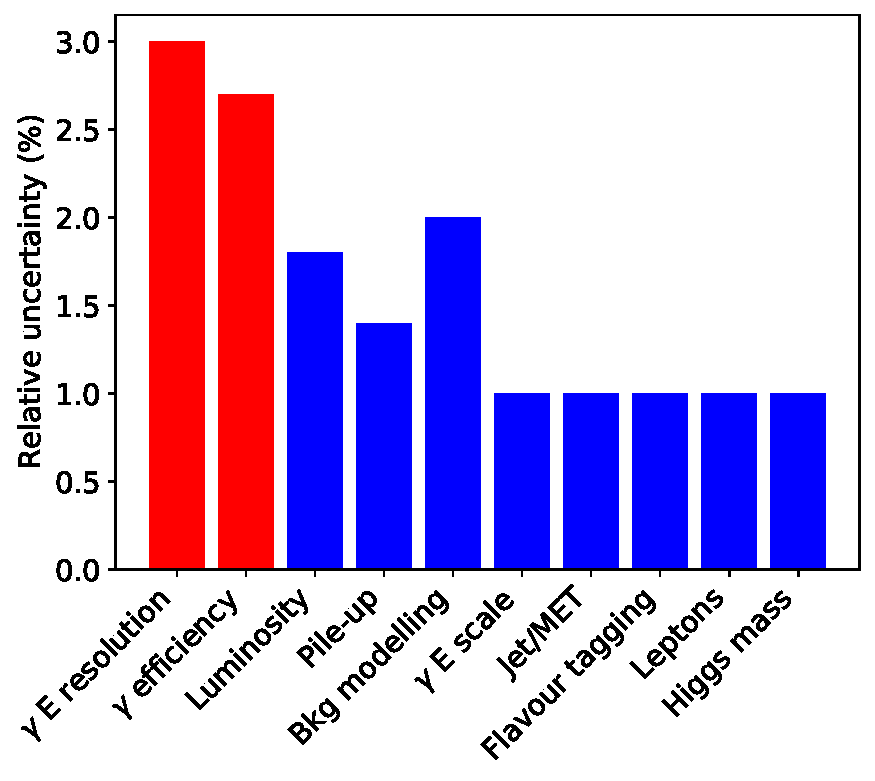
\includegraphics[width=0.45\textwidth]{figures/ggFbbarbH_syst.pdf}}
  \subfigure[\tth]{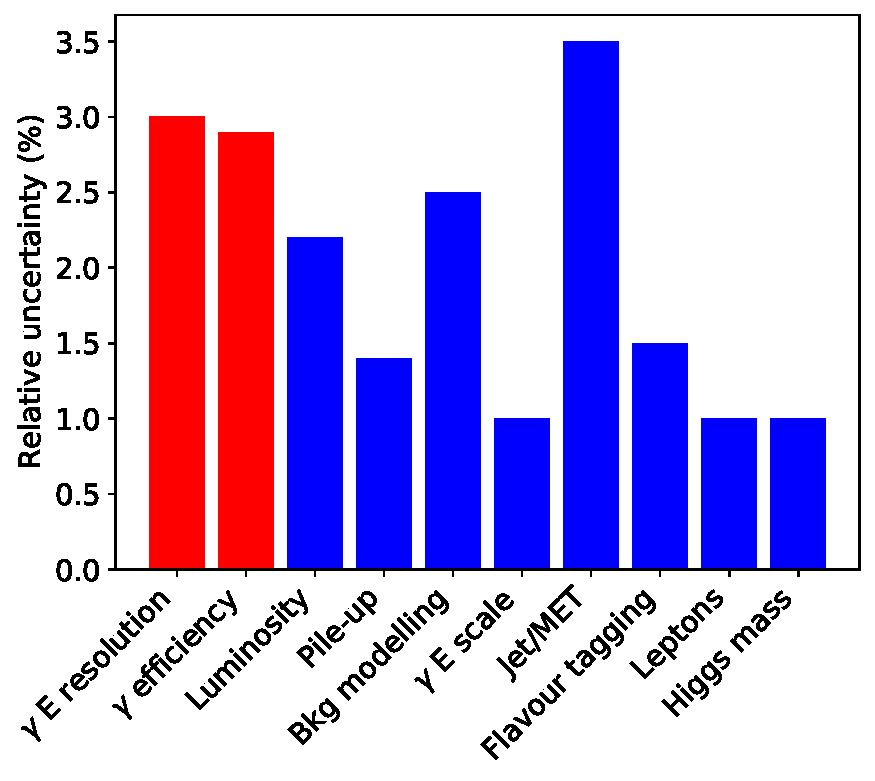
\includegraphics[width=0.45\textwidth]{figures/tth_syst.pdf}}
  \caption{\label{fig:stxs_unc} Expected contributions from the main sources of experimental systematic uncertainty to the total uncertainty in the measurement of the cross-section times $H\to\gamma\gamma$ branching ratio for gluon-gluon fusion Higgs production and \tth\ processes~\cite{ATLAS_STXS}. The uncertainty from each source is shown as a fraction of the total expected cross-section ($\sigma$). The magnitude of these uncertainties grows significantly for the differential cross section measurements (up to a total of {\color{red} X\%})}
\end{figure}

% How will reducing the uncertainties which are already small (for the total)? How will reducing differential cross sections improve SMEFT and kappa results

% What is my unique contribution that makes the proposal greater than the sum of its parts (1+1>2)
% What about the ongoing anomaly detection work?
% ANL trigger (HLT) work?
% Speed up the calibration loop?
% Anomaly detection and calibration: can anomalies identified with ML be used to make calibrations more robust?

\section{Project Objectives}
The objective of the proposed work is to gain experience with decorrelation techniques for calibration tasks and to build a framework to easily deploy such methods for various calibration tasks. These approaches can help incorporate calibration considerations (e.g., differences between recorded data and simulation) into ML models which will result in a decrease in uncertainties. This will maximize the power of precision measurements by improving physics object ID and energy evaluation. This approach will first be applied to the ATLAS photon ID and energy resolution calibration which will in turn be used in the upcoming \hyy, focusing on \tthyy, differential cross section measurements. Decorrelation techniques will also be used in the optimization of \hyy\ measurements by ensuring that final multivariate analysis (MVA) does not change the background $\gamma\gamma$ spectrum. The decorrelation framework will then be integrated into existing ATLAS ML frameworks such as ``salt''~\cite{salt}.
% Mention "salt"
\begin{itemize}
\item Develop method to incorporate calibration considerations into ML physics object ID
  \begin{itemize}
  \item Using recent decorrelation schemes
  \end{itemize}
\item Apply decorrelation techniques to calibrate photon ID efficiency and photon energy 
\item Study the use of clustering for automated calibration binning
\item Perform updated \tthyy\ differential cross section measurement with improved photon ID and resolution
\item Integrate framework into existing ATLAS ML frameworks
\end{itemize}

\section{Proposed Research and Method}
% Gordon's talk on training with variables  https://indico.in2p3.fr/event/30589/contributions/130476/attachments/81700/120373/2023-11-30%20Using%20Adversaries%20to%20Control%20Systematics.pdf

% Photon ID
% - Join efforts (describe them) that is attempting to use ML for photon ID
% - Apply decorrelation technique
% - Work on calibration including using clustering
% - Collaborate to see if the same technique can be applied at the HLT

% Photon resolution
% - Join existing efforts (describe them) that are using GNNs
% - Study the use of adversarial techniques to avoid data/MC differences
% - Work on calibration including using clustering
% - HLT for sharper turn ons

% HL-LHC?
% Beyond the LHC?
% Auto calibration

% How does this connect to other work and ANL?
% - Anomaly detection


The PI's team, consisting of two postdocs at 2.0 FTE, will customize and deploy decorrelation techniques to improve photon energy and photon ID calibration. The two general approaches, decorrelation and adversarial, will be studied in parallel by the two postdocs, with one postdoc gaining expertise in adversarial techniques and the other in decorrelation methods which will have the same application and thus input features, data, and caveats.

The decorrelation techniques will first be applied to ML calibration and ID approaches using BDTs and will then be adapted to be used with more nascent and advanced networks such as GNNs. The adversarial approaches as well as GNNs require significant computing resources to train and tune. The PI will make use of the computing resources at Argonne via the Laboratory Computing Resources Center (LCRC) and the resources and expertise at Argonne Leadership Computing Facility (ALCF). The Argonne ATLAS group already has a renewing computing allocation at LCRC which includes a cluster (six nodes with eight graphical processing units, GPUs, each) that will be used to build models that include decorrelation. Additional resources and expertise is available at the ALCF which includes both NVIDIA and Itel GPU resources. The PI's team will make use of previous connections with ALCF experts to help develop and train the decorrelation approaches on ALCF resources. Allocations for these resources will be requested as they are needed.

The photon energy and ID calibrations will then be used for full Run 3 $H\to\gamma\gamma$ STXS measurement. The PI's team will focus on the \tth\ measurement drawing from previous experience with final states that include $\ttbar$ within Supersymmetry searches and more recently, final states that include two photon final states within a charged Higgs search. 

Once the proposed approaches have been developed and validated for photons, the PI's team will work members of the Argonne ATLAS group (who will not funded by this proposal, if awarded), who are involved in flavor tagging, to study the decorrelation techniques for other ID tasks.

% Finally, the PI and members of the Argonne ATLAS group are also working on using anomaly detection for error detection at the HLT.
% Not sure how the anomaly detection is linked to calibration


\subsection{Photon energy calibration}

% Add short description of the calibration:
% Input: shower variables
% Output: Energy
% Figure of merit: difference between truth particle energy and output use MAE
% Good general reference that explains unbinned calibration:
% https://indico.cern.ch/event/789893/contributions/3281009/attachments/1780367/2896144/MCcal_17012019.pdf

Photon and electron energy is calibrated using several steps which are detailed in~\cite{atlascollaboration2023electron}.
The MC-based calibration, which this proposal seeks to use as a test case and to improve, uses variables derived from groupings of energy deposits in the calorimeter and aims to correct for the energy lost in the material upstream of the calorimeter, for the energy deposited in the cells neighbouring the cluster, and the energy lost beyond the LAr calorimeter. The current algorithm uses a BDT to regress the corrected photon energy using shower-related variables that summarize shower properties (see Figure~\ref{fig:showerVars}). The BDT is trained with a single particle MC with a flat transverse momentum (\pt) spectrum up to 150 GeV. The performance of the BDT is then evaluated by comparing the energy predicted by the BDT with the true particle energy. Internal ATLAS studies have shown that adding lateral shower shape variables to the BDT could improve the energy resolution after calibration by 10-15\%. However, these variables are poorly modelled by the simulation when compared to recorded data, preventing them from being used in the calibration. Including data or simulations that has been weighted to mimic data distributions together with decorrelation techniques could recover some of the improvements resulting from including shower shape variables without being affected by data/MC differences.

\begin{figure}[ht]
  \centering
  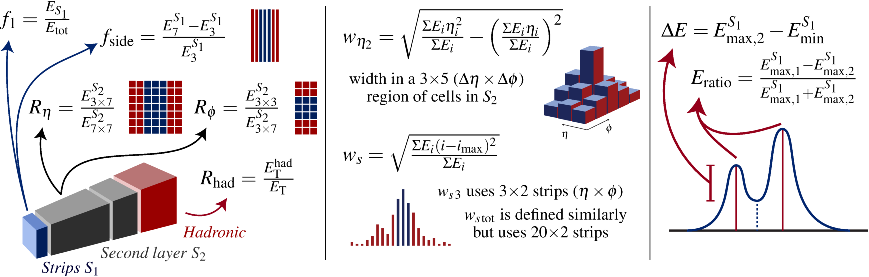
\includegraphics[width=\textwidth]{figures/photon_ID_variables.pdf}
  \caption{\label{fig:showerVars} }
\end{figure}

% Why not just reweight MC to look more like data during training?
% - When training on data, this could reduce uncertainty, no?
% - How do you get the data?
% - You only care about data/MC differences in the important quantity. Thus adding this difference should give you the optimal and most robust model
% - What about pileup
% Check why Gordon didn't just do this?
The two decorrelation methods will be studied in parallel, first on the photon energy calibration using the existing BDT energy regression, and then using a more advanced approach that utilizes GNNs and low-level calorimeter information. The PI's team will apply the methods studied by the PI on a simplified toy example and described in ~\cite{} using the existing BDT. One postdoc will focus on the adversarial technique while the other will focus on the decorrelation approach, each at 0.5 FTE. The current BDT does not suffer from large discrepancies between data and simulations but studies within ATLAS have shown that adding additional variables, specifically quantities that describe the shower shape, which are poorly modelled in simulations could improve the performance of the BDT. The BDT has been extensively studied for various improvements and will serve as a benchmark to ensure that the mismodeling reducing (i.e., decorrelation) techniques do not effect the original ML algorithm in a negative way.

% Who will work with me on this?
The PI's team will first, together with ATLAS $e/\gamma$, produce a simulation data set that has been modified to resemble the data. This ``fudged'' MC will allow for more control of properties such as photon purity, energy scale, and sample size for initial studies; the team will also study the use of data during training after the decorrelation models reach a mature state. The team will use the previously developed toy model as a basis to develop decorrelation methods for the energy regression BDT. As a former convener of the ATLAS Full Simulation group, which aims to improve both the physics and computational performance of the ATLAS detector simulation based on GEANT4~\cite{Agostinelli:2002hh}, the PI will also work with the Full Simulation experts to revisit understanding the source of the mismodelling.

% Transfer learning -> go from fudged MC to data or other mild mismodelling

The figure of merit for determining the best decorrelation approach will the energy resolution. However, the framework developed to apply these methods will be carried over for use on more complex ML calibrations. The approach that results in the best physics performance, i.e., with the lowest 50\% interquartile range, and with the best data/MC agreement will be chosen for further validation and integration into the ATLAS $e/\gamma$ photon calibration procedure.

% Don't really need k-means for binning, no?

A GNN-based calibration is being developed by the University of Edinburgh, University of California at Berkeley, Lawrence Berkeley National Laboratory, and Michigan State University, and has shown promise in improving the photon energy resolution significantly (up to 20\%). However, the calibration resulting from the GNN-based approach differs for data and MC. The PI's team with collaborate with the GNN calibration team to introduce decorrelation approaches to the powerful GNN calibration.

\subsection{Photon identification}

The ATLAS photon identification utilizes similar quantities to what are used for the photon energy calibration, of which some are highlighted in Figure~\ref{fig:showerVars}. Unlike the photon energy calibration, the ATLAS photon ID does not make use of a multivariate approach. This is mainly due to the calibration procedure for the photon ID, which requires the ID algorithm to be independent of the isolation. The decorrelation techniques, that this proposal aims to develop, may be the key to moving the photon ID to a multivariate technique such as a BDT or approaches that use low-level variables such as GNNs. Once the move to multivariate methods is possible, the decorrelation can be extended to minimize data-MC difference as proposed for the photon energy calibration.

The PI's team will work closely with photon reconstruction experts at Northern Illinois University (NIU) who have previously studied the use of BDTs and convolutional neural networks (CNNs) for photon identification, members of the ALCF data science group who have studied PointCloud~\cite{ATL-PHYS-PUB-2021-002} NNs for object ID to develop a multivariate photon ID method, and other ATLAS collaborators who have used ML approaches for photon ID. The decorrelation techniques will first be applied to a BDT or NN that takes high-level quantities as inputs, similar to those currently used in the cut-based approach. As with the energy resolution calibration, both the decorrelation and adversarial techniques will be studied in parallel by the two postdocs of the team. Once the output of the multivariate technique has been shown to be independent of the isolation, the team will work to fully calibrate the new ID algorithm using the standard techniques described in~\cite{PERF-2013-04,PERF-2017-02}.

The experienced gained from applying the decorrelation techniques on a high-level inputs will be used to apply similar methods to a GNN that uses low-level, i.e., energy deposits in the calorimeter cells, inputs.

Finally, the photon ID algorithm will be trained with fudged MC to make it more robust against mismodelling, as was done with the photon energy estimation. 

\subsection{\tthyy}
\begin{wrapfigure}{l}{0.5\textwidth}
  \centering
  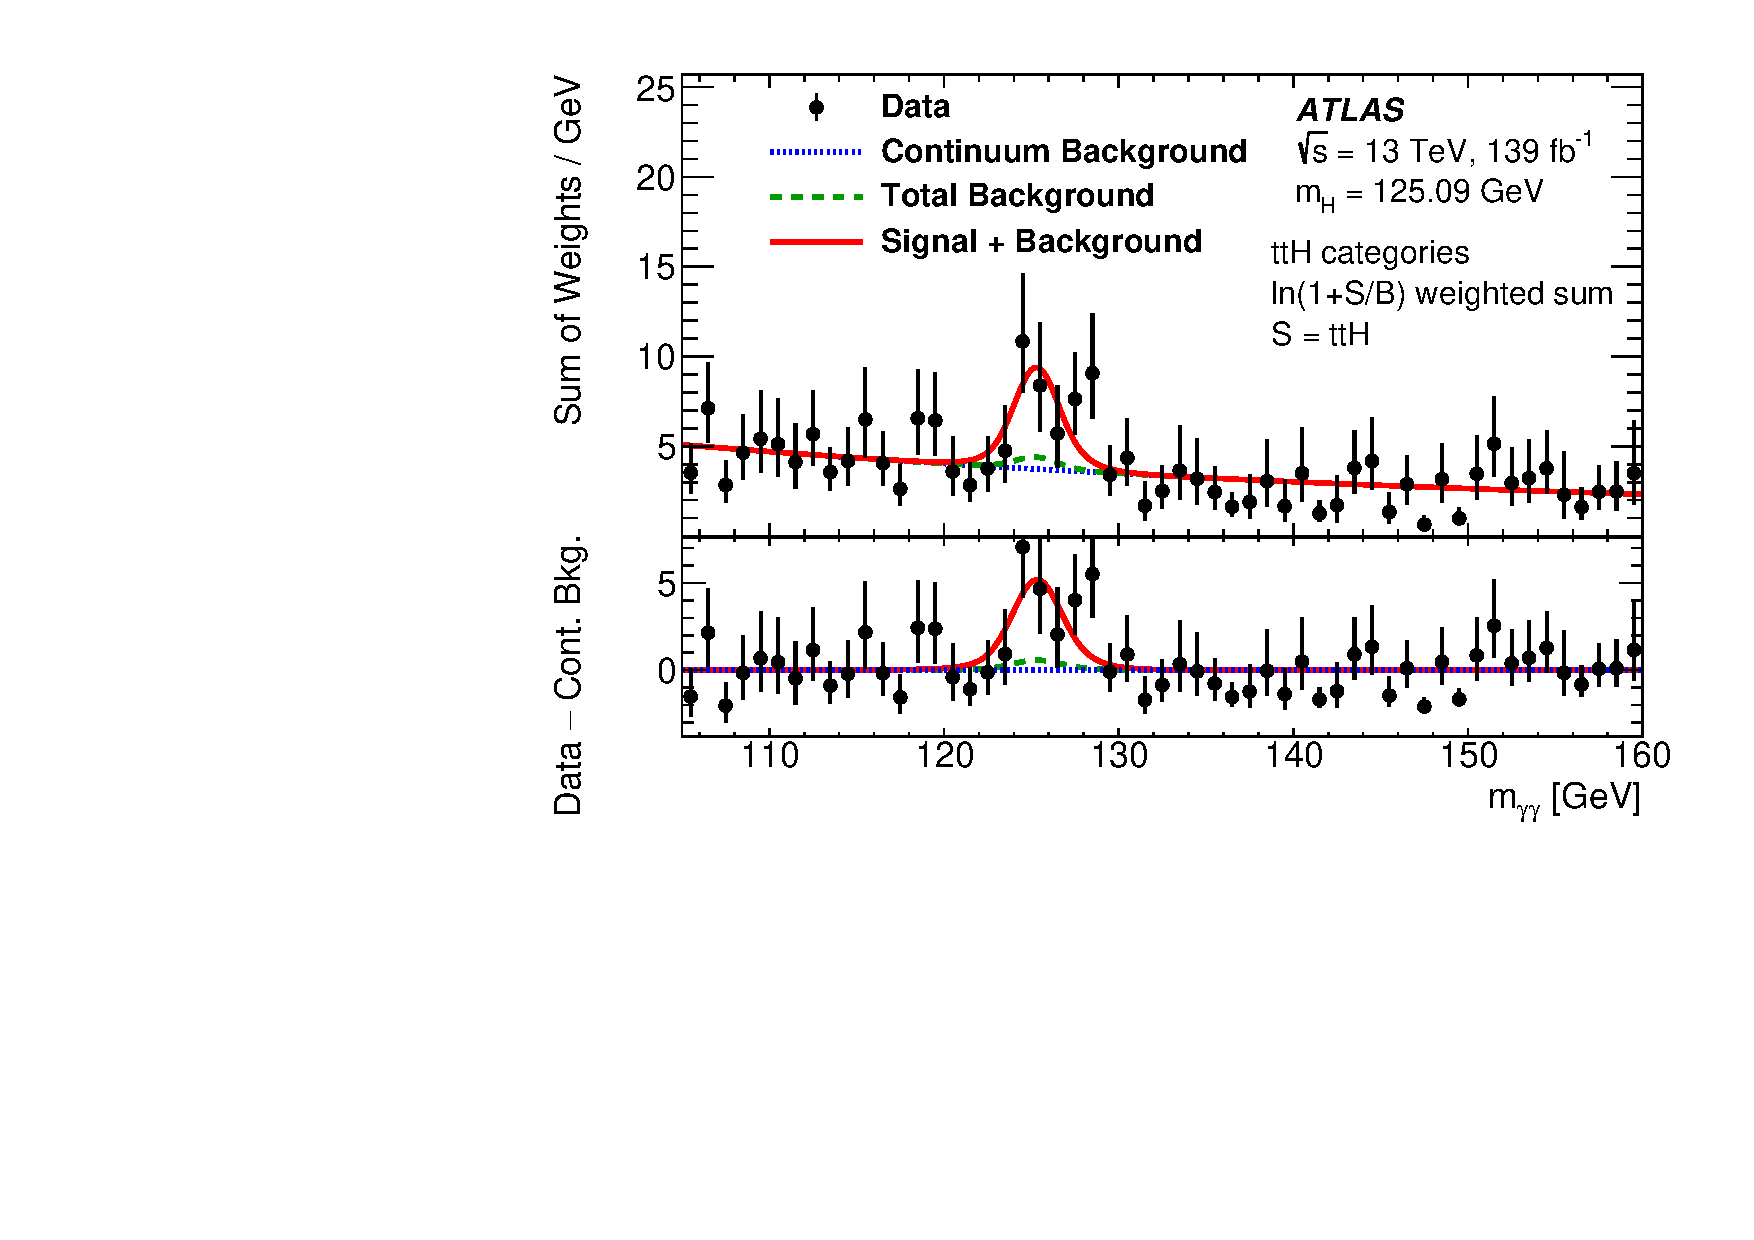
\includegraphics[width=\linewidth]{figures/tth_myy.pdf}
  \caption{\label{fig:myy} Distribution of the diphoton invariant mass in the \ttH\ channel for the latest STXS ATLAS result~\cite{ATLAS_STXS}. The data (dots) is shown together with the sum of the fitted signal plus background (solid line). The blue dotted line represents the sum of the fitted continuum background, while the dashed line combines the contributions of continuum background and other Higgs boson events.}
\end{wrapfigure}

The most recent ATLAS results that performed many differential cross section measurements in the \hyy\ channel made use of BDTs to both discriminate between the differential cross section bins and to separate background from signal processes. One of the main background in many channels is the continuum diphoton background which is estimated using a functional fit to the \myy\ spectrum (see Figure~\ref{fig:myy} for an example). Due to this background estimation methodology, only variables that were found to have less than a 5\% linear correlation with the \myy\ spectrum were used in the BDT training. The decorrelation techniques to improve the photon calibration can also be used to ensure that an ML classifier is independent of the \myy\ spectrum. This application of decorrelation approaches is similar to techniques that have been proposed to decorrelate algorithms to identify substructure within a jet from the mass of the jet, allowing the technique to be used for any mass of a hypothesised BSM particle.

Using the framework that was developed for the photon ID MVA and energy calibration, the two postdocs will work in parallel to determine which decorrelation approach, decorrelation versus adversarial, is optimal for ensuring that the diphoton invariant mass spectrum remains uncorrelated with the signal-to-background MVA (either a BDT or NN). The method that both ensures that the background shape remains unchanged and results in the highest signal significance, which will now take advantage of more variables, will be first used in the \ttH\ channel and then will be extended to other channels.

The PI's team will also contribute to the final interpretations of the \hyy\ result. The two interpretations, each of which will be performed by one of the postdocs and the PI, are withing the $\kappa$-modifier framework and the SMEFT. 


\subsection{Timetable of Activities}
\label{sec:timetable}
% Always consider the master timeline:
% https://lhc-commissioning.web.cern.ch/schedule/LHC-long-term.htm

The timetable of activities is shown in Figure~\ref{fig:timetable}.
\begin{figure}[!htbp]
  \centering
  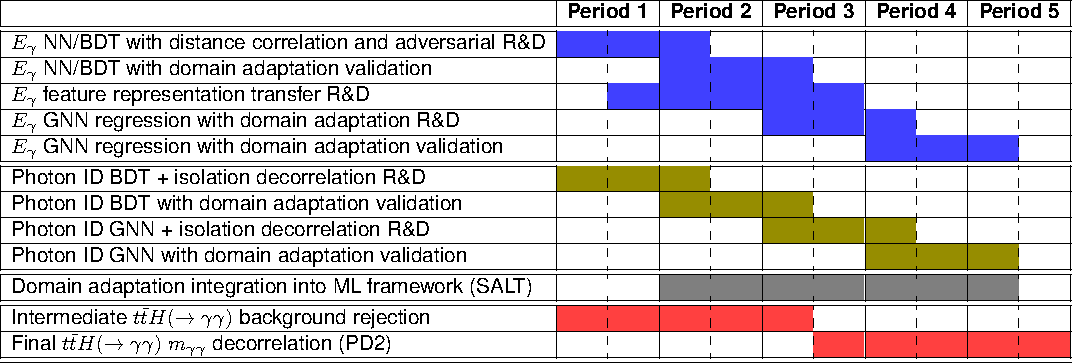
\includegraphics[width=\textwidth]{figures/timeline.pdf}
  \caption{Expected time spent on the work proposed in this text by the PI's team which will consists of two postdocs (at 1.0 FTE each) and about half of the PI's effort. Each period is 12 months long with Period 1 starting on August 1st 2024 and Period 5 ending on July 31st 2029 which is two months after the HL-LHC is slated to start operations (May 2029). 
  }
  \label{fig:timetable}
\end{figure}

Below is a summary of the milestones:
\begin{enumerate}
\item Finalization of framework that can apply both decorrelation as well as adversarial methods to decorrelate multivariate algorithms from certain quantities. 
\item Reduction in photon energy resolution uncertainty due to decorrelation of data/MC differences.
\item Multivariate photon ID that is decorrelated from isolation
  % \item Photon ID uncertainty reduced due to decorrelation of data/MC differences
\item Improved background rejection in \ttH\
\item SMEFT and $\kappa$ interpretation of \ttH\ result
\end{enumerate}



\subsection{Personnel and Resources}
\label{sec:personnel}
The PI will lead a team to conduct the proposed work, which will consist of an average of 2.0 postdoctoral FTEs and 50\% of the PI's effort.

The postdocs, covered 100\% by this award, is expected to start work at the beginning of the first Period. Both postdocs will be work on the proposed projects until Period 5. The postdoc's time will be split between developing decorrelation approaches and preparing the new \tthyy\ result. 

The PI will also collaborate with graduate and undergraduate students on the proposed research, through the DOE Office of Science Graduate Student Research program and the Science Undergraduate Laboratory Internships, respectively. Furthermore, Argonne's ATLAS Center, which hosts graduate students from universities that are members of the ATLAS collaboration, provides other opportunities to collaborate on the proposed work. The PI will work with students from institutions with established collaborations with the Argonne ATLAS group, such as NIU. NIU has both photon and Higgs expertise but also has a computing traineeship which has synergies with this proposal due to the computing required to perform the proposed research.

Computing resources available at the ALCF include Polaris (which is an NVIDIA GPU farm) and Aurora (which has Intel GPUs). The resources are available to the PI in the form of Director's Discretionary Allocations, which are routinely granted with consideration to clearly defined specifications. An additional computing resource for smaller-scale testing will also be available through the Laboratory Computing Resource Center.

%The PI's team expects to collaborate with \GEANT\ experts and the ATLAS simulation team, ATLAS SUSY group members, and ALCF computing experts. The PI has already established these collaborations by working within the ATLAS simulation optimization task force, leading SUSY analyses, and working with ALCF in the context of the ATLAS Aurora ESP, respectively. 

\section{Summary}


\clearpage

\appendix
\part*{Appendices}
% \renewcommand\thesection{\Roman{section}}
\addcontentsline{toc}{part}{Appendices}
\section{Biographical sketch}
\centerline{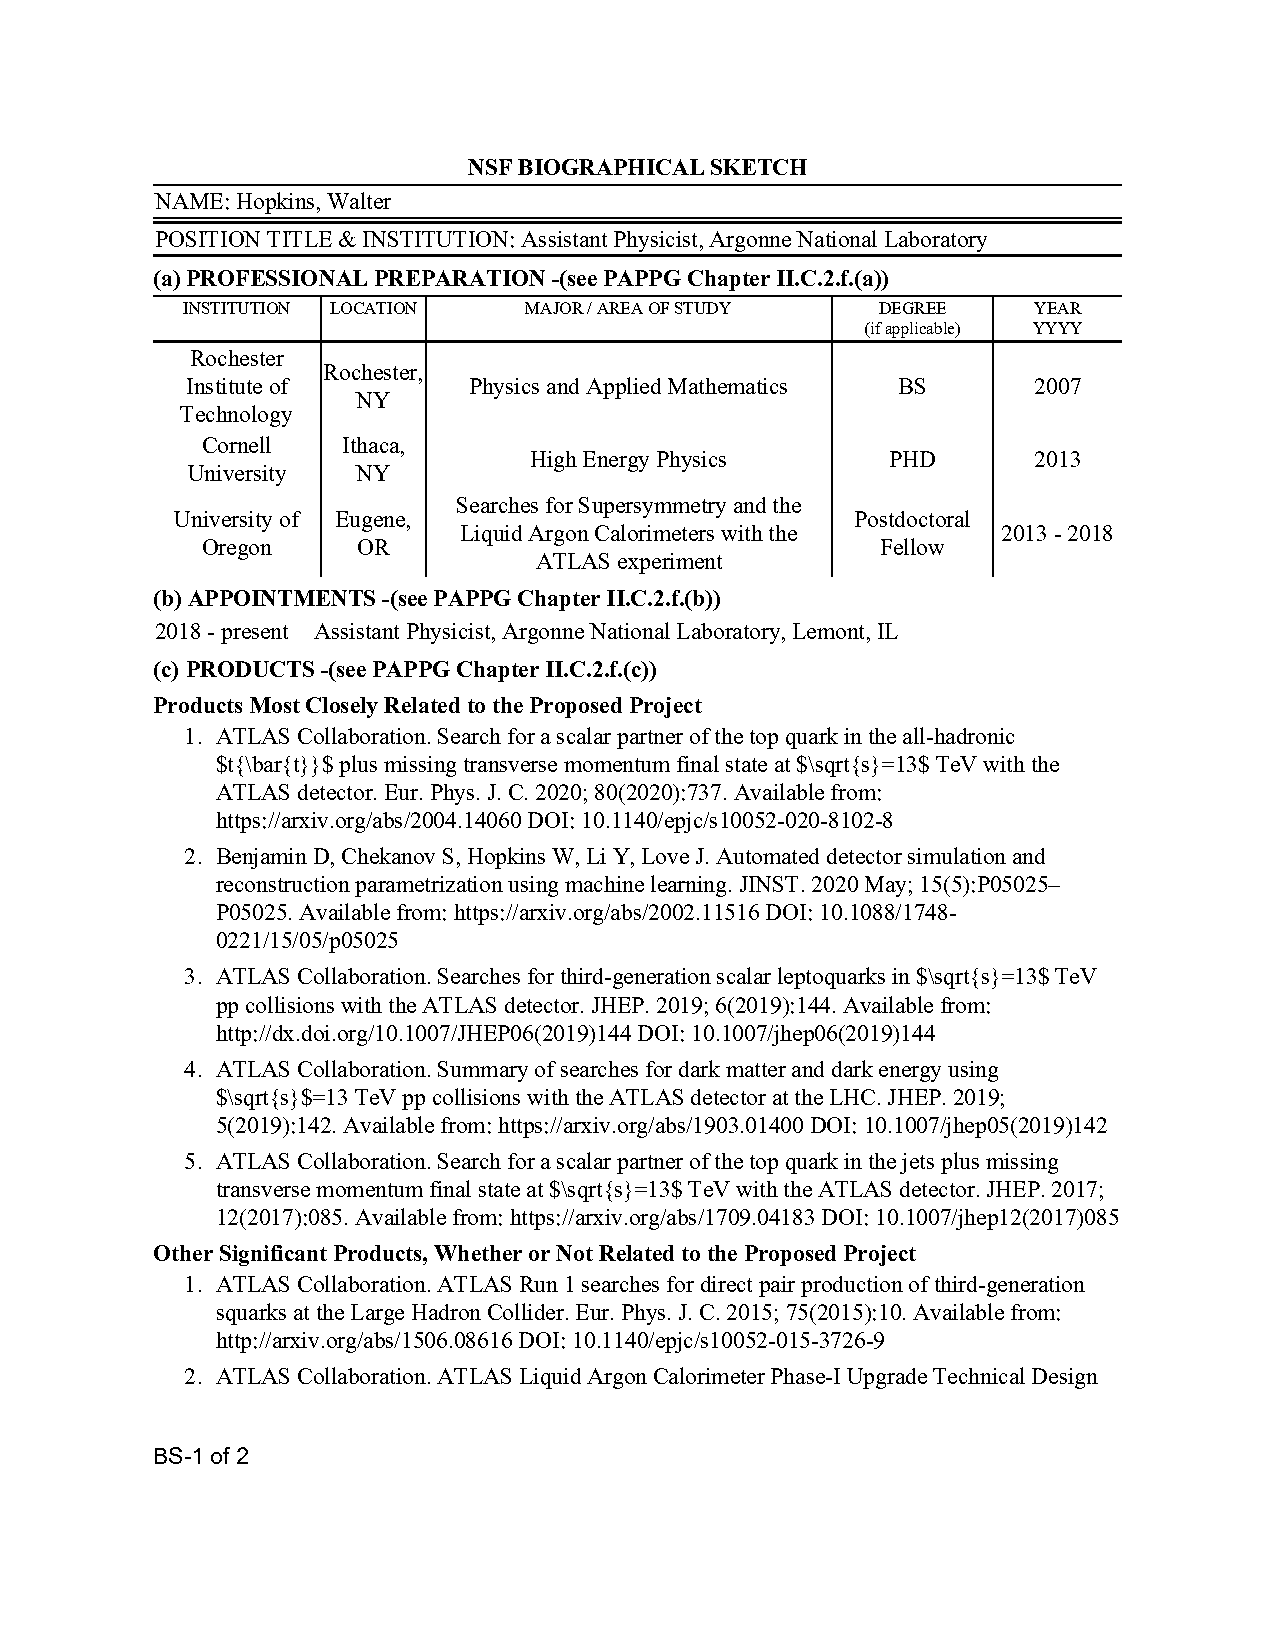
\includegraphics[width=0.99\paperwidth,trim=0 1.73in 0 1.06in,clip]{bioSketch.pdf}}
\includepdf[scale=1,pages=2-,trim=0 1.76in 0 1.06in,clip,pagecommand={}]{bioSketch.pdf}

\clearpage

% \includepdf[scale=.96,pages={1},trim=0 1.5in 0 1.06in,clip,pagecommand=\section{Current and pending support}]{cps_filled.pdf}
% \includepdf[scale=1,pages=2-,trim=0 1.5in 0 1.06in,clip,pagecommand={}]{cps_filled.pdf}
% \clearpage

\printbibliography[title={Bibliography and References},heading=bibnumbered]
\clearpage

\section{Facilities and  other resources}
Argonne offers various resources, including office space for postdocs and potential students as well as several computing resources. The computing resources expected to be utilized include CPU and GPU resources available through the Laboratory Computing Resource Center at Argonne. These resources are expected to be used to produce input data for ML algorithms as well as training the ML algorithms. The PI also plans to use computing resources at the ALCF resources, such as Polaris (which has NVIDIA GPUs) and Aurora (which contains Intel GPUs), via a discretionary allocation. These resources will be used for large-scale training and optimization of the proposed approach.

An additional important resource is the ATLAS experiment at the LHC at CERN. The PI's team will make use of ATLAS data and simulation for the proposed studies and will occasionally travel to CERN to work with international collaborators.

\clearpage

\section{Equipment}
The requested funding will be used to purchase three laptops for the postdocs that the PI will supervise. The combined cost of the three laptops is expected to be \$8,524.

\clearpage

\section{Data management plan}
The majority of the data and code produced will come from the ATLAS experiment. ATLAS has its own data management plan which the PI's team will adhere to; the details of that plan can be found at \url{https://po.usatlas.bnl.gov/programoffice/datamanagementpolicy.php}.

Scientific results that used ATLAS data will be published in a scientific journal or an ATLAS publication note, which will be publicly available on \url{https://arxiv.org/} and \url{https://twiki.cern.ch/twiki/bin/view/AtlasPublic/SimulationPublicResults}, respectively. Figures and tables will be made available in the same way as other ATLAS results, via HEPData (\url{https://www.hepdata.net/}) and ATLAS public pages. 

Additional data that are produced outside of ATLAS for initial ML algorithm development will be stored on the Argonne High Energy Physics divisional nodes in the HDF5 format and will consist of energy deposits in a simplified detector. The generated data are expected to occupy a small fraction of the available data storage on these nodes. Code and configurations used for the development of the algorithm and production of data will be kept at the Argonne Computing, Environment and Life Sciences (CELS) gitlab repository: \url{https://xgitlab.cels.anl.gov/}. Results from these studies, if published, will be publicly available on \url{https://arxiv.org/}. 

\clearpage

\section{Promoting Inclusive and Equitable Research (PIER) Plan}

\clearpage

\section{Recruitment and Retention of Students and Early-stage Investigators}

\clearpage

\section{Other attachments}
There are no other attachments.

\end{document}
